\documentclass{sig-alternate-2013}

\setlength{\paperheight}{11in}
\setlength{\paperwidth}{8.5in}

\usepackage[utf8]{inputenc}

\usepackage{amsmath,amssymb}
\usepackage{amsthmnoproof}
\usepackage{amsrefs}
\usepackage[usenames,dvipsnames]{color}
\usepackage{stmaryrd}
\usepackage{enumerate}
\usepackage[algoruled,vlined,english,linesnumbered]{algorithm2e}
\usepackage[pdfpagelabels,colorlinks=true,citecolor=blue]{hyperref}
\usepackage{comment}
\usepackage{multirow}
\usepackage{tikz}

\newcommand{\noopsort}[1]{}
\DeclareMathOperator{\NP}{NP}
\DeclareMathOperator{\HP}{HP}
\DeclareMathOperator{\PP}{PP}
\DeclareMathOperator{\Hom}{Hom}
\DeclareMathOperator{\End}{End}
\DeclareMathOperator{\GL}{GL}
\DeclareMathOperator{\val}{val}
\DeclareMathOperator{\pr}{pr}
\DeclareMathOperator{\tr}{Tr}
\DeclareMathOperator{\com}{Com}
\DeclareMathOperator{\Grass}{Grass}
\DeclareMathOperator{\Lat}{Lat}
\DeclareMathOperator{\round}{round}
\DeclareMathOperator{\rank}{rank}

\newcommand{\slp}{\text{\rm slp}}
\newcommand{\RS}{\text{\rm RS}}

\newcommand{\N}{\mathbb N}
\newcommand{\Z}{\mathbb Z}
\newcommand{\Zp}{\Z_p}
\newcommand{\Q}{\mathbb Q}
\newcommand{\Qp}{\Q_p}
\newcommand{\Fp}{\mathbb{F}_p}
\newcommand{\R}{\mathbb R}
\renewcommand{\O}{\mathcal O}
\newcommand{\OK}{\mathcal{O}_K}
\newcommand{\XX}{\mathbf X}
\newcommand{\trans}{{}^{\text t}}
\newcommand{\T}{\mathcal{T}}

\renewcommand{\prec}{\text{\rm prec}}
\newcommand{\NF}{\text{\rm NF}}

\renewcommand{\mod}{\,\%\,}
\renewcommand{\div}{\,/\hspace{-0.3em}/\,}
\newcommand{\nfop}[1]{%
\raisebox{-0.1mm}{\begin{tikzpicture}
\draw[transparent] (-0.18,0)--(0.18,0);
\draw[very thin] (0,0) circle (0.11cm);
\begin{scope}
\clip (0,0) circle (0.11cm);
\node[scale=0.75] at (0,0) { $#1$ };
\end{scope}
\end{tikzpicture}}}
\newcommand{\nfplus}{\nfop+}
\newcommand{\nftimes}{\nfop\times}
\newcommand{\nfmod}{\nfop\mod}
\newcommand{\nfdiv}{\nfop\div}

\newcommand{\id}{\textrm{id}}
\newcommand{\Epi}{\textrm{Epi}}
\renewcommand{\c}{\text{\rm c}}

\newcommand{\detp}{\det{'}}
\newcommand{\low}{\text{\rm low}}
\newcommand{\up}{\text{\rm up}}
\newcommand{\DI}{\text{\rm DI}}
\newcommand{\II}{\text{\rm II}}
\DeclareMathOperator{\charpoly}{char}
\newcommand{\charp}{\charpoly'}

\newcommand{\lb}{\ensuremath{\llbracket}}
\newcommand{\rb}{\ensuremath{\rrbracket}}
\newcommand{\lp}{(\!(}
\newcommand{\rp}{)\!)}
\newcommand{\col}{\: : \:}

\newcommand{\tinyplus}{\raisebox{0.4mm}{\hspace{0.4mm}\tiny +\hspace{0.4mm}}}

\def\todo#1{\ \!\!{\color{red} #1}}
\definecolor{purple}{rgb}{0.6,0,0.6}
\def\todofor#1#2{\ \!\!{\color{purple} {\bf #1}: #2}}

\def\binom#1#2{\Big(\begin{array}{cc} #1 \\ #2 \end{array}\Big)}


\permission{%
}



\begin{document}

\newtheorem{theo}{Theorem}[section]
\newtheorem{lem}[theo]{Lemma}
\newtheorem{prop}[theo]{Proposition}
\newtheorem{cor}[theo]{Corollary}
\newtheorem{quest}[theo]{Question}
\newtheorem{conj}[theo]{Conjecture}
\theoremstyle{definition}
\newtheorem{rem}[theo]{Remark}
\newtheorem{ex}[theo]{Example}
\newtheorem{deftn}[theo]{Definition}

\title{Division and Factorization of p-Adic Polynomials}

\numberofauthors{3}
\author{
\alignauthor Xavier Caruso\\
  \affaddr{Universit\'e Rennes 1}\\
  \affaddr{\textsf{xavier.caruso@normalesup.org}}
\alignauthor David Roe \\
  \affaddr{University of Pittsburgh}\\
  \affaddr{\textsf{roed.math@gmail.com}}
\alignauthor Tristan Vaccon\\
  \affaddr{Rikkyo University}\\
  \affaddr{\textsf{vaccon@rikkyo.ac.jp}}
}

\maketitle

\begin{abstract}
\end{abstract}

\category{I.1.2}{Computing Methodologies}{Symbolic and Algebraic Manipulation -- \emph{Algebraic Algorithms}}
\terms{Algorithms, Theory}
\keywords{}

%\vspace{1mm}
% \noindent
% {\bf Categories and Subject Descripto\RS:} \\
%\noindent I.1.2 [{\bf Computing Methodologies}]:{~} Symbolic and Algebraic
%  Manipulation -- \emph{Algebraic Algorithms}
%
% \vspace{1mm}
% \noindent
% {\bf General Terms:} Algorithms, Theory
%
% \vspace{1mm}
% \noindent
% {\bf Keywords:} $p$-adic precision, linear algebra, ultrametric analysis
%\medskip

\section{Introduction}

\noindent
{\bf Notations.}
Throughout this paper, we fix a complete discrete valuation field $K$; 
we denote by $\val : K \to \Z \cup \{+\infty\}$ the valuation on it and 
by $W$ its ring of integers (\emph{i.e.} the set of elements with 
nonnegative valuation). We assume that $\val$ is normalized so that it
is surjective and denote by $\pi$ a uniformizer of $K$, that is an 
element of valuation $1$. Denoting by $S \subset W$ a fixed set of 
representatives of the classes modulo $\pi$ and assuming $0 \in S$, 
one can prove that each element in $x \in K$ can be represented 
uniquely as a convergent series:
\begin{equation}
\label{eq:CDVFseries}
x = \sum_{i=\val(x)}^{+\infty} a_i \pi^i
\quad \text{with} \quad a_i \in S.
\end{equation}
The two most important examples are the field of $p$-adic numbers $K = 
\Qp$ and the field of Laurent series $K = k((t))$ over a field $k$. The 
valuation on them are the $p$-adic valuation and the usual valuation of 
a Laurent series respectively. Their ring of integers are therefore 
$\Zp$ and $k[[t]]$ respectively. A distinguished uniformizer is $p$ 
and $t$ whereas a possible set $S$ is $\{0, \ldots, p-1\}$ and $k$
respectively.
The reader who is not familiar with complete discrete valuation fields
may assume (without sacrifying too much to the generality) that $K$ is
one of the two aforementioned examples.

In what follows, the notation $K[X]$ refers to the ring of univariate 
polynomials with coefficients in $K$. The subspace of polynomials of 
degree at most $n$ (resp. exactly $n$) is denoted by $K_{\leq n}[X]$ 
(resp. $K_{=n}[X]$).

\section{Precision data}

Elements in $K$ (and \emph{a fortiori} in $K[X]$) carry an infinite 
amount of information. They thus cannot be stored entirely in the
memory of a computer and have to be truncated. Elements of $K$ are
usually represented by truncating Eq.\eqref{eq:CDVFseries} as
follows:
\begin{equation}
\label{eq:CDVFseriesO}
x = \sum_{i=v}^{N-1} a_i \pi^i + O(\pi^N)
\end{equation}
where $N$ is an integer called the \emph{absolute precision} and 
the notation $O(\pi^N)$ means that the coefficients $a_i$ for $i
\geq N$ are discarded. If $N > v$ and $a_v \neq 0$, the integer $v$ 
is the valuation of $x$ and the difference $N-v$ is called the
\emph{relative precision}.
Alternatively, one may thing that the writing~\eqref{eq:CDVFseriesO}
represents a subset of $K$ which consists of all elements in $K$ for
which the $a_i$'s in the range $[v,N-1]$ are those specified. From the
metric point of view, this is a ball (centered at any point inside it).

It worths be noting that tracking precision using this representation is 
rather easy. For example, if $x$ and $y$ are known with absolute (resp. 
relative) precision $N_x$ and $N_y$ respectively, one can compute the 
sum $x+y$ (resp. the product $xy$) at absolute (resp. relative) 
precision $\min(N_x,N_y)$. Computations with $p$-adic and Laurent
series are often handle this way on symbolic computation softwares.

\subsection{Precision for polynomials}

The situation is much more subtle when we are working with a collection 
of elements of $K$ (\emph{e.g.} a polynomial) and not just a single one.
Indeed, several precision data may be considered and, as we shall see
later, each of them has is own interest. Below we detail three of them
for the special case of polynomials.

\medskip

\noindent
{\bf Jagged precision.}
The most naive precision we may consider is the so-called \emph{jagged 
precision}. It consists in attaching an individual precision (of the
shape $O(\pi^{N_i})$) to each coefficient separatedly.

\medskip

\noindent
{\bf Newton precision.} 
We now move to \emph{Newton precision} data. They can be actually seen 
as particular instances of jagged precision but there exist for them 
better representations and better algorithms.

\begin{deftn}
A \emph{Newton function of degree $n$} is a convex function 
$\varphi : [0,n] \to \R \cup \{+\infty\}$ which is piecewise affine, 
which takes a finite value at $n$ and whose epigraph $\Epi(\varphi)$ 
have integral extremal points.
\end{deftn}

\begin{rem}
The datum of $\varphi$ is equivalent to that of $\Epi(\varphi)$ and they 
can easily represented and manipulated on a computer.
\end{rem}

We recall that one can attach a Newton function to each polynomial.
If $P(X) = \sum_{i=0}^n a_n X^n \in K_n[X]$, we define its Newton
polygon $\NP(P)$ as the convex hull of the points $(i,\val(a_i))$ 
($1 \leq i \leq n$) together with the point at infinity $(0,+\infty)$
and then its Newton function $\NF(P) : [0,n] \to \R$ as the unique
function whose epigraph is $\NP(P)$. It is well known \todo{(Give a
reference?)} that:
$$\begin{array}{r@{\,\,}c@{\,\,}l}
\NP(P+Q) & \subset & \text{Conv}\big(\NP(P) \cup \NP(Q)\big) \smallskip \\
\NP(PQ) & = & \NP(P) + \NP(Q)
\end{array}$$
where $\text{Conv}$ denotes the convex hull and the plus sign stands 
for the Minkowski sum. This translates to:
$$\begin{array}{r@{\,\,}c@{\,\,}l}
\NF(P+Q) \geq \NF(P) \nfplus \NF(Q) \smallskip \\
\NF(PQ) = \NF(P) \nftimes \NF(Q)
\end{array}$$
where the operations $\nfplus$ and $\nftimes$ are defined accordingly.
There exist classical algorithms for computing these two operations
whose complexity is quasi-linear with respect to the degree.

In a similar fashion, Newton functions can be used to model precision: 
given a Newton function $\varphi$ of degree $n$, we agree that a polynomial 
of degree at most $n$ is given at precision $O(\varphi)$ when, for all $i$,
its $i$-th coefficient is given at precision $O\big(\pi^{\lceil \varphi(i)
\rceil}\big)$ (where $\lceil \cdot \rceil$ is the ceiling function).
In the sequel, we shall write
$O(\varphi) = \sum_{i=0}^n O\big(\pi^{\lceil \varphi(i) \rceil}\big) \cdot X^i$
and use the notation $\sum_{i=0}^n a_i X^i + O(\varphi)$ (where the
coefficients $a_i$ are given by truncated series) to refer to a 
polynomial given at precision $O(\varphi)$.

It is easily checked that if $P$ and $Q$ are two polynomials known at 
precision $O(\varphi_P)$ and $O(\varphi_Q)$ respectively, then $P+Q$ is 
known at precision $O(\varphi_P \nfplus \varphi_Q)$ and $PQ$ is known at 
precision $O\big((\varphi_P \nftimes \NF(Q)) \nfplus (\NF(P) \nftimes 
\varphi_Q)\big)$.

\begin{deftn}
\label{def:nondeg}
Let $P = P_0 + O(\varphi_P)$. We say that the Newton precision 
$O(\varphi_P)$ on $P$ is \emph{nondegenerate} if $\varphi_P \geq 
\NF(P_0)$ and $\varphi_P(x) > y$ for all extremal point $(x,y)$ of 
$\NP(P_0)$.
\end{deftn}

We notice that, under the conditions of the above definition, the
Newton polygon of $P$ is well defined. Indeed, if $\delta P$ is any
polynomial whose Newton function is not less than $\varphi_P$, we
have $\NP(P_0 + \delta P) = \NP(P_0)$.

\medskip

\noindent
{\bf Lattice precision.}
The notion of \emph{lattice precision} was developed in 
\cite{padicprec}. It encompasses the two previous models and has
the decisive advantage of optimality. As a counterpart, it might be
very space-consuming and time-consuming for polynomials of large
degree.

\begin{deftn}
Let $V$ be a finite dimensional vector space over $K$. A lattice
in $V$ is a sub-$W$-module of $V$ generated by a $K$-basis of
$V$.
\end{deftn}

\noindent
We fix an integer $n$. A lattice precision datum for a polynomial of 
degree $n$ is a lattice $H$ lying in the vector space $K_{\leq n}[X]$. 
We shall sometimes denote it $O(H)$ in order to emphasize that it should 
be considered as a precision datum. The notation $P(X) + O(H)$ then 
refers to any polynomial in the $W$-affine space $P(X) + H$. Tracking
lattice precision can be done using differentials as shown in
\cite[Lemma~3.4 and Proposition~3.12]{padicprec}: if $f : K_{\leq n}[X] 
\to K_{\leq m}[X]$ denotes any strictly differentiable function with
surjective differential, under mild assumption on $H$, we have:
$$f(P(X)+H) = f(P(X)) + f'(P(X))(H)$$
where $f'(P(X))$ denotes the differential of $f$ at $P(X)$. The
equality sign reflets the optimality of the method.

As already mentioned, the jagged precision model is a particular case of 
the lattice precision. Indeed, a precision of the shape $\sum_{i=0}^n 
O(\pi^{N_i}) X^i$ corresponds to the lattice generated by the elements 
$\pi^{N_i} X^i$ ($0 \leq i \leq n$). This remark is the origin of the 
notion of \emph{diffused digits of precision} introduced in 
\cite[Definition 2.3]{preclinalg}. We shall use it repeatedly in the 
sequel in order to compare the behaviour of the three aforementioned 
precision data in concrete situations.

\section{Euclidean division}

\todo{Add introduction.}
In the sequel, we shall will the notation $A \div B$ (resp $A \mod B$)
for the quotient (resp. the remainder) in the Euclidean division of $A$ 
by $B$.

\subsection{Euclidean division of Newton functions}

\begin{deftn}
Let $\varphi$ and $\psi$ be two Newton functions of degree $n$ and
$d$ respectively. Letting $\mu = \psi(d) - \psi(d-1)$ and $\Delta$
be the greatest affine function of slope $\mu$ with $\Delta \leq
\varphi$, we define:
$$\begin{array}{rcl}
\varphi \nfmod \psi \, : \, [0, d-1] & \to & \R \cup \{+\infty\} \smallskip \\
x & \mapsto & \psi(x) + \Delta(d) - \psi(d) \medskip \\
\varphi \nfdiv \psi \, : \, [0, n-d] & \to & \R \cup \{+\infty\} \smallskip \\
x & \mapsto & \inf_{h \geq 0} \psi(x+d+h) - \mu h.
\end{array}$$
\end{deftn}

\begin{figure}
\hfill
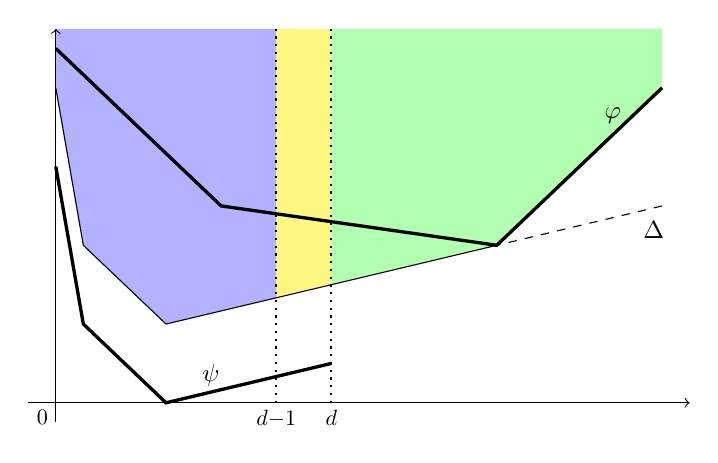
\begin{tikzpicture}[xscale=0.7, yscale=0.5]
\fill[blue!30] (4,9.5)--(4,2.667)--(2,2)--(0.5,4)--(0,8)--(0,9.5)--cycle;
\fill[yellow!50] (5,9.5)--(5,3)--(4,2.667)--(4,9.5)--cycle;
\fill[green!30] (5,9.5)--(5,3)--(8,4)--(11,8)--(11,9.5)--cycle;
\draw[->] (-0.5,0)--(11.5,0);
\draw[->] (0,-0.5)--(0,9.5);
\draw[very thick] (0,6)--(0.5,2)--(2,0)--(5,1);
\draw[very thick] (0,9)--(3,5)--(8,4)--(11,8);
\draw[dashed] (11,5)--(8,4);
\draw (8,4)--(2,2)--(0.5,4)--(0,8);
\draw[dotted,thick] (5,0)--(5,9.5);
\draw[dotted,thick] (4,0)--(4,9.5);
\node[scale=0.8, below left] at (0,0) { $0$ };
\node[scale=0.8, below] at (5,0) { $d$ };
\node[scale=0.8, below] at (4,0) { $d{-}1$ };
\node[scale=0.9, below right] at (2.5,1.2) { $\psi$ };
\node[scale=0.9, right] at (9.8,7.3) { $\varphi$ };
\node[scale=0.9, right] at (10.5,4.4) { $\Delta$ };
\end{tikzpicture}
\hfill \null

\vspace{-6mm}

\caption{Euclidean division of Newton functions}
\label{fig:NewtonEuclide}
\end{figure}

Figure~\ref{fig:NewtonEuclide} illustrates the definition: if $\varphi$ 
and $\psi$ are the functions represented on the diagram, the epigraph of 
$\varphi \nfmod \psi$ is the blue area whereas that of $\varphi \nfdiv \psi$ 
is the green area translated by $(-d,0)$.
It is an easy exercise (left to the reader) to design algorithms for
computing $\varphi \nfmod \psi$ and $\varphi \nfdiv \psi$ for a cost
which is at most $n + O(1)$.

\begin{theo}
\label{theo:EDivisionNP}
Let $A, B \in K[X]$ with $B \neq 0$. Let $d$ be the degree of $B$.
Let $\mu = \NF(B)(d) - \NF(B)(d{-}1)$ be the last slope of $B$ and 
$y = \Delta(x)$ be the
equation of the highest line of slope $\mu$ lying below $\NP(A)$.
Then:
\begin{align}
\NF(A \mod B) & \geq \NF(B) \nfmod \NF(A) \label{eq:AmodB} \\
\text{and} \hspace{4mm}
\NF(A \div B) & \geq \NF(B) \nfdiv \NF(A) \label{eq:AdivB}
\end{align}
\end{theo}

\begin{rem}
Keeping the notations of the Theorem and decomposing $A$ as a sum 
$A_{<d} + A_{\geq d}$ where $A_{<d}$ (resp. $A_{\geq d}$) consists of
monomials of $A$ of degree $< d$ (resp of degree $\geq d$), we have:
$$A \div B = A_{\geq d} \div B 
\quad \text{and} \quad
A \mod B = A_{<d} + (A_{\geq d} \mod B).$$
Using the above relations and applying Theorem~\ref{theo:EDivisionNP}
with $A_{\geq d}$ and $B$ (instead of $A$ and $B$ respectively) may lead
to a better lower bound on the Newton function of $A \div B$ and $A \mod
B$.
\end{rem}

\begin{proof}[of Theorem~\ref{theo:EDivisionNP}]
Let us first prove Eq.~\eqref{eq:AmodB}. 
Replacing $B$ by $c^{-1} B$ where $c$ denotes the leading coefficient
of $B$, we may assume that $B$ is monic. Using linearity, we may further
assume that $A$ is a monomial. Set $R_n = X^n \mod B$. The relation
we have to prove is:
$$\NF(R_n)(x) \geq \NF(B)(x) - \mu(n-d).$$
When $n < d$, we have $R_n = 0$ and the assertion of the Theorem holds. 
For larger $n$, we proceed by induction. We have the relation
$R_{n+1} = X R_n - c_n B$
where $c_n$ is the coefficient in $X^{d-1}$ of $R_n$. Thanks to the
induction hypothesis, we have:
\begin{align*}
\val(c_n) \geq \NF(R_n)(d{-}1) & \geq \NF(B)(d{-}1) - \mu(n{-}d) \\
& = - \mu(n{+}1{-}d)
\end{align*}
since $\mu = -\NF(B)(d{-}1)$ because $B$ is monic. Therefore
$\NF(c_n B)(x) \geq \NF(B)(x) - \mu(n+1-d)$ for all $x$. On the 
other hand, for all $x$, we have:
$$\NF(X R_n)(x) = \NF(R_n)(x{-}1) \geq \NF(R_n)(x) - \mu$$
from what we get $\NF(X R_n)(x) \geq \NF(B)(x) - \mu(n+1-d)$. As a
consequence
$\NF(R_{n+1})(x) \geq \NF(B)(x) - \mu(n+1-d)$
and the induction follows.
Eq.~\eqref{eq:AdivB} is now derived from:
$$\NF(A \div B) \nftimes \NF(B) \geq \NF(A) \nfplus \NF(A \mod B)$$
using the estimation on $\NF(A\mod B)$ we have just proved
(see Figure~\ref{fig:NewtonEuclide}).
\end{proof}

\subsection{Tracking precision}

\medskip

\noindent
{\bf Jagged precision.}
\todo{Write something... Explain in particular that the fast methods
(based on fast multipliction) may lead to important looses of precision.}

\medskip

\noindent
{\bf Newton precision.}
We consider here the case where the precision is given by Newton
functions. Concretely, we pick $A, B \in K[X]$ two polynomials which 
are known at precision $O(\varphi_A)$ and $O(\varphi_B)$ respectively:
$$A = A_0 + O(\varphi_A)
\quad \text{and} \quad
B = B_0 + O(\varphi_B)$$
Here $A_0$ and $B_0$ are some approximations of $A$ and $B$ respectively 
and $\varphi_A$ and $\varphi_B$ denotes two Newton functions of degree 
$\deg A$ and $\deg B$ respectively.
We are interesting in determining the precision on $A \mod B$ and $A
\div B$. The following proposition gives a theoretical answer under
mild assumptions.

\begin{prop}
\label{prop:NewtonprecEuclide}
We keep the above notations and assume that the Newton precisions
$O(\varphi_A)$ and $O(\varphi_B)$ on $A$ and $B$ respectively are 
both nondegenerate (\emph{cf} Definition~\ref{def:nondeg}). Then,
setting:
$$\varphi = \varphi_A \nfplus 
\big[ \varphi_B \nftimes \big(\NF(A) \nfdiv \NF(B)\big) \big]$$
the polynomials $A \div B$ and $A \mod B$ are known at precision 
$O(\varphi \nfdiv \NF(B))$ and $O(\varphi \nfmod \NF(B))$ respectively.
\end{prop}

\begin{proof}
Let $\delta A$ (resp. $\delta B$) be a polynomial whose Newton 
function is not less than $\varphi_A$ (resp. $\varphi_B$) and define
$\delta Q$ and $\delta R$ by:
\begin{align*}
Q_0 + \delta Q & = (A_0 + \delta A) \div (B_0 + \delta B) \\
R_0 + \delta R & = (A_0 + \delta A) \mod (B_0 + \delta B)
\end{align*}
where $Q_0 = A_0 \div B_0$ and $R_0 = A_0 \mod B_0$.
We have to show that $\NF(\delta Q) \geq \varphi \nfdiv \NF(B)$ and
$\NF(\delta R) \geq \varphi \nfmod \NF(B)$.
Set $\delta X = \delta A - Q_0 \delta B$. 
Using Theorem~\ref{theo:EDivisionNP}, we obtain $\NF(Q_0) \geq
\NF(A) \div \NF(B)$ and consequently $\NF(\delta X) \geq \varphi$.
On the other hand, an easy computation yields
$$\delta X = (B + \delta B) \cdot \delta Q + \delta R$$
so that $\delta Q = \delta X \div (B + \delta B)$ and 
$\delta R = \delta X \mod (B + \delta B)$. Using again 
Theorem~\ref{theo:EDivisionNP}, we get the desired result.
\end{proof}

\todo{Explain how one can use this proposition: we split the computation
into two parts (approximation and precision)...\\
Don't forget to give the complexity.}

\medskip

\noindent
{\bf Lattice precision.}
We now move to lattice precision. We pick $A$ and $B$ two polynomials 
of respective degree $n$ and $d$ and assume that they are known at 
precision $O(H_A)$ and $O(H_B)$ respectively:
$$A = A_0 + O(H_A)
\quad \text{and} \quad
B = B_0 + O(H_B).$$
where $H_A \in K_{\leq n}[X]$ and $H_B \in K_{\leq d}[X]$ are lattices. 
According to the results of \cite{padicprec}, in order to determine the 
precision on $A \div B$ and $A \mod B$, we need to compute the 
differential of the mappings $(X,Y) \mapsto X \div Y$ and $(X,Y)
\mapsto X \mod Y$ at the point $(A_0, B_0)$. Writing $Q_0 = A_0 \div
B_0$ and $R_0 = A_0 \mod B_0$, this can be done by
expanding the relation:
$$A_0 + dA = (B_0 + dB) (Q_0 + dQ) + (R_0 + dR)$$
and neglecting the terms of order $\geq 2$. We get this way 
$dA = B_0 dQ + Q_0 dB + dR$
meaning that $dQ$ and $dR$ appears respectively as the quotient and
the remainder of the Euclidean division of $dX = dA - B_0 dQ$ by $B_0$.

Once this has been done, the strategy is quite similar to that explained 
for Newton precision: \todo{summerize this in one sentence.}

\subsection{An example: modular multiplication}

For this example, we work over $W = \Z_2$ and fix a monic polynomial $M 
\in \Z[X]$ (known exactly) of degree $5$. Our aim is to compare the 
numerical stability of the multiplication in the quotient $\Z_2[X]/M(X)$ 
depending on the precision model we are using. In order to do so, we 
pick $n$ random polynomials $P_1, \ldots, P_n$ in $\Z_2[X]/M(X)$ 
(according to the Haar measure) whose coefficients are all known at 
precision $O(2^N)$ for some large integer $N$. We then compute the 
product of the $P_i$'s using the following quite naive algorithm.

\noindent\hrulefill

%\noindent {\bf Algorithm 1:} {\tt example\_product}
%
%\smallskip

\noindent 1.\ {\bf set} $P = 1$

\noindent 2.\ {\bf for} $i=1,\dots,n$ {\bf do} {\bf compute} $P = (P 
\cdot P_i) \mod M$

\noindent 3.\ {\bf return} $P$

\vspace{-1ex}\noindent\hrulefill

\medskip

The table below reports the average gain of \emph{absolute} 
precision $G$ which is observed while executing the algorithm above 
for various modulus and $n$. The average is taken on a sample of $1000$ 
random inputs. We recall that $G$ is defined as follows:

\noindent $\bullet$
in the case of jagged and Newton precision, the precision on the output 
may be written into the form $\sum_{i=1}^4 O(2^{N_i}) \: X^i$ and 
$G = \sum_{i=1}^4 (N_i - N)$;

\noindent $\bullet$
in the case of lattice precision, the precision on the output is a 
lattice $H$ and $G$ is the index of $H$ in $2^N \mathcal L$ where 
$\mathcal L = \Z_2[X]/M$ is the standard lattice; in that case, we write 
$G$ as a sum $G_{\text{nd}} + G_{\text{d}}$ where $G_{\text{d}}$ is the 
index of $H$ in the largest lattice $H_0$ contained in $H$ which can be 
generated by elements of the shape $2^{N_i} X^i$ ($0 \leq i \leq 4$). 
(The term $G_d$ corresponds to diffused digits according to 
\cite[Definition 2.3]{preclinalg}.)

\medskip

{\small%
\noindent \hfill%
\renewcommand{\arraystretch}{1.2}%
\begin{tabular}{|c|c|c|c|c|}%
\hline
\multirow{3}{*}{Modulus $M$} & 
\multirow{3}{*}{\hspace{2mm}$n$\hspace{2mm}} & 
\multicolumn{3}{c|}{Gain of precision} \\
\cline{3-5}
& & \multirow{2}{*}{Jagged} & \multirow{2}{*}{Newton}
      & \raisebox{-0.5mm}{Lattice} \\
& & & & \raisebox{0.5mm}{\scriptsize (not dif.\tinyplus dif.)} \\
\hline
\multirow{3}{*}{\begin{tabular}{@{}c@{}} $X^5 + X^2 + 1$ \\ {\scriptsize (Irred. mod $2$)} \end{tabular}}
& $10$ & $\phantom{00}0.2$ & $\phantom{00}0.2$ & $\phantom{00}0.2\tinyplus\phantom{00}0.0$ \\
& $50$ & $\phantom{00}4.2$ & $\phantom{00}4.2$ & $\phantom{00}4.2\tinyplus\phantom{00}0.0$ \\
& $100$ & $\phantom{0}11.2$ & $\phantom{0}11.2$ & $\phantom{0}11.2\tinyplus\phantom{00}0.0$ \\
\hline
\multirow{3}{*}{\begin{tabular}{@{}c@{}} $X^5 + 1$ \\ {\scriptsize (Sep. mod $2$)} \end{tabular}}
& $10$ & $\phantom{00}0.4$ & $\phantom{00}0.4$ & $\phantom{00}0.9\tinyplus\phantom{00}6.0$ \\
& $50$ & $\phantom{00}5.6$ & $\phantom{00}5.6$ & $\phantom{0}11.1\tinyplus\phantom{0}42.0$ \\
& $100$ & $\phantom{0}13.6$ & $\phantom{0}13.6$ & $\phantom{0}27.0\tinyplus\phantom{0}87.0$ \\
\hline
\multirow{3}{*}{\begin{tabular}{@{}c@{}} $X^5 + 2$ \\ {\scriptsize (Eisenstein)} \end{tabular}}
& $10$ & $\phantom{00}6.2$ & $\phantom{00}6.2$ & $\phantom{00}6.2\tinyplus\phantom{00}0.0$ \\
& $50$ & $\phantom{0}44.0$ & $\phantom{0}44.0$ & $\phantom{0}44.0\tinyplus\phantom{00}0.0$ \\
& $100$ & $\phantom{0}92.5$ & $\phantom{0}92.5$ & $\phantom{0}92.5\tinyplus\phantom{00}0.0$ \\
\hline
\multirow{3}{*}{\begin{tabular}{@{}c@{}} $(X+1)^5 + 2$ \\ {\scriptsize (Shift Eisenstein)} \end{tabular}}
& $10$ & $\phantom{00}0.6$ & $\phantom{00}0.6$ & $\phantom{00}4.7\tinyplus\phantom{00}1.4$ \\
& $50$ & $\phantom{00}7.1$ & $\phantom{00}7.1$ & $\phantom{0}42.6\tinyplus\phantom{00}1.4$ \\
& $100$ & $\phantom{0}15.1$ & $\phantom{0}15.1$ & $\phantom{0}91.8\tinyplus\phantom{00}1.4$ \\
\hline
\multirow{3}{*}{\begin{tabular}{@{}c@{}} $X^5 + X + 2$ \\ {\scriptsize (Two slopes)} \end{tabular}}
& $10$ & $\phantom{00}1.7$ & $\phantom{00}1.7$ & $\phantom{00}7.9\tinyplus\phantom{00}9.8$ \\
& $50$ & $\phantom{00}8.1$ & $\phantom{00}8.1$ & $\phantom{0}70.7\tinyplus\phantom{0}59.8$ \\
& $100$ & $\phantom{0}16.1$ & $\phantom{0}16.1$ & $152.6\tinyplus125.9$ \\
\hline
\end{tabular}
\hfill \null}

\medskip

We observe several interesting properties. First of all, the gains for 
Newton precision and jagged precision always agree though one may has 
thought at first that Newton precision is weaker. Since performing
precision computations in the Newton framework is cheaper, it seems
(at least on this example) that using the jagged precision model is not
relevant.

On the other hand, the lattice precision may end up with better results. 
Nevertheless this strongly depends on the modulus $M$. For instance, 
when $M$ is irreducible modulo $p=2$ or Eiseistein, there is apparently 
no benefit of using the lattice precision model. We emphasize that 
these two particular cases correspond to modulus that are usually used 
to define (unramified and totally ramified respectively) extensions of 
$\Q_2$.

For other modulus, the situation is quite different and the benefit of 
using the lattice precision model becomes more apparent. 
The comparison between the gain of precision in the jagged model and 
the number of not diffused digits in the lattice model makes sense:
indeed the latter appears as a theoretical upper bound of the former
and the difference between them quantifies the quality of the way we
track precision in the jagged (or the Newton) precision model. We 
observe that this difference is usually not neglictible (\emph{cf} 
notably the case of $M(X) = (X+1)^5 + 2$) meaning that this quality 
is not very good in general.
As for diffused digits, they correspond to digits that cannot be 
``seen'' in the jagged precision model. Their number then measures the 
intrinsic limitations of this model. We observe that it can be very 
important as well in several cases.

\todo{Add some words about the comparison between $X^5 + 2$ and
$(X+1)^5 + 2$?}

\section{Slope factorization}

A well-known theorem \todo{(Give a reference?)} asserts that each 
extremal point $M$ in the Newton polygon $\NP(P)$ of a polynomial $P \in 
K[X]$ corresponds to a factorization $P = AB$ where the Newton polygon 
of $A$ (resp. $B$) is given by the part of $\NP(P)$ located at the left 
(resp. the right) of $M$. Such a factorization is often called a 
\emph{slope factorization}.

The aim of this section is to design efficient and stable algorithms 
for computing these factorizations. \todo{Compare with previous
results...}

\subsection{A Newton iteration}

In the previous references, the factor $A$ defined above is always 
obtained \emph{via} a Newton iteration which takes place over a finite 
extension of $K$. We introduce here a variant of this Newton iteration 
whose main advantage to be defined over $K$ itself.

\begin{theo} \label{theo:slope-factor}
Let $P(X) = \sum_{i=0}^n a_i X^i$ be a polynomial of degree $n$ with
coefficients in $K$. We assume that $\NP(P)$ has an extremal point 
whose abscissa is $d$.
We define the sequences $(A_i)_{i \geq 0}$ and $(V_i)_{i \geq 0}$
recursively by:
\begin{align*}
A_0 & = \sum_{i=0}^d a_i X^i, \quad V_{0} = 1 \medskip \\
A_{i+1} &= A_i + (V_i P \:\mod\: A_i), \smallskip \\
V_{i+1} &= (2 V_i -V_i^2 B_{i+1} ) \mod A_{i+1} \\
& \hspace{2cm}\text{where } B_{i+1} = P \div A_{i+1}.
\end{align*}
Then the sequence $(A_i)$ convergences to a divisor $A$ of $P$ 
of degree $d$ whose leading coefficient is $a_d$ and whose Newton 
function agrees with $\NF(P)$ on $[0,d]$.
\end{theo}

%\begin{rem}
%Using $P \mapsto P^*=X^{deg(P)}P \left( \frac{1}{X} \right), $ the assumptions in Theorem \ref{theo:slope-factor} do not induce any loss in generality.
%\end{rem}

%\begin{rem}
%Non necessity to have $A_0$ as the first slope. It is possible to use minorations.
%
%\begin{tikzpicture}
%\draw[->] (0,-1) -- (0,2);
%\draw[->] (-0.05,0) -- (4,0);
%\node[left] at (0,0) {$0$};
%\draw (1.5,-.1) -- (1.5,.1);
%\node[above] at (1.5,0) {$d$};
%\draw (0,1)-- (1.5,0) -- (3,-.375)-- (3.5,.625);
%\draw[green] (0,1.5)-- (1,0.33)-- (1.5,0) --(2,-.125)-- (3,0)-- (3.5,1);
%\node[below] at (.75,-0.2) {$\lambda_0$};
%\end{tikzpicture}
%\end{rem}

\begin{rem}
The divisor $A$ is uniquely determined by the conditions of 
Theorem~\ref{theo:slope-factor}.
\end{rem}

The rest of this subsection is devoted to the proof of the theorem.
If $d = n$ (resp. $d = 1$), the sequence $A_i$ is constant equal to
$P$ (resp. to the constant coefficient of $P$) and theorem is clear.
We then assume $1 < d < n$. Without loss of generality, we may further 
assume that the coefficient $a_d$ is equal to $1$. We set:
\begin{align*}
\lambda_0 & = \NF(P)(d) - \NF(P)(d{-}1) \\
\lambda_1 & = \NF(P)(d{+}1) - \NF(P)(d).
\end{align*}
The existence of an extremal point of $\NP(P)$ located at abscissa
$d$ ensures that $\lambda_1 > \lambda_0$.
For all indices $i$, we define:
$$\begin{array}{r@{\,\,}lr@{\,\,}l}
Q_i &= V_i P \div A_i, &
R_i & = V_i P \mod A_i = A_{i+1} - A_i, 
\smallskip \\
S_i &= P \mod A_i, &
T_i &= 1 - V_i B_i. 
\end{array}$$
and when $\square$ is some letter, we put $\Delta \square_i = \square_{i+1} 
- \square_i$.
%We use the next Lemma to record some useful formulae.

\begin{lem} \label{lem:formulae}
The following relations hold:
\begin{align}
\Delta B_i &= -(R_i B_{i+1}) \div A_i, \label{eqdef:Biminus} \\
\Delta S_i &= -(R_i B_{i+1}) \mod A_i,  \label{eqdef:Siminus} \\
S_{i} &= (B_i R_i + T_i S_{i-1} - T_i \: \Delta S_{i-1}) \mod A_{i}, \label{eqdef:Si2}  \\
\Delta V_i &= (V_i T_i - V_i^2 \: \Delta B_i) \mod A_{i}, \label{eqdef:Viminus}\\
1-Q_i &= T_i + (R_i-V_i S_i) \div A_i, \label{eqdef:Qiminus}\\
R_{i+1} &= (\Delta V_i \: S_{i+1}+(1{-}Q_i)R_i) \mod A_{i+1}, \label{eq:Riplus}\\
T_{i+1} &\equiv T_i + V_i \: (\Delta B_i)^2 \pmod{A_{i+1}}. \label{eq:ViBiplus}
\end{align}
\end{lem}

\begin{proof}
From $P= A_i B_i + S_i= A_{i+1} B_{i+1} + S_{i+1}$, we get
$- R_i B_{i+1}= \Delta B_i \cdot A_i + \Delta S_i$.
Hence, by consideration of degree, we obtain \eqref{eqdef:Biminus} 
and \eqref{eqdef:Siminus}.
On the other hand, from $V_i P = A_i Q_i + R_i=V_i (A_i B_i + S_i)$, we 
derive
\begin{equation}
\label{eq:ViBiQi} 
(V_i B_i -Q_i) \cdot A_i=R_i-V_i S_i. 
\end{equation} 
Thus $R_i=V_i S_i \mod A_i$.
Hence $B_i R_i = (S_i - S_i T_i) \mod A_i$ and $S_i = B_i R_i + S_i T_i 
\mod A_i$, from what \eqref{eqdef:Si2} follows directly.
By definition of $V_i$, we get $\Delta V_i = V_i (1-V_i B_{i+1}) \mod A_{i+1}$ and consequently \eqref{eqdef:Viminus}.
We now write $1-Q_i= T_i + (V_i B_i - Q_i)$. Using \eqref{eq:ViBiQi}, we 
get \eqref{eqdef:Qiminus}.

We have $V_i P=A_i Q_i+R_i=(A_{i+1}-R_i)Q_i+R_i$ and $V_{i+1} P=A_{i+1} 
Q_{i+1}+R_{i+1}$. Thus:
\begin{align*}
R_{i+1} &= \Delta V_i \: P + (1-Q_i)R_i \\
 &= (\Delta V_i \: S_{i+1} + (1-Q_i)R_i) \mod A_{i+1},
\end{align*} 
and \eqref{eq:Riplus} is proved. Finally
\begin{align*}
T_{i+1} &\equiv 1-2V_i B_{i+1}+V_i^2 B_{i+1}^2 \pmod {A_{i+1}} \\
&\equiv (1-V_i B_{i+1})^2 \pmod {A_{i+1}} \\
&\equiv T_i + V_i (\Delta B_i)^2 \pmod {A_{i+1}}
\end{align*}
which concludes the proof.
\end{proof}

\begin{deftn}
Notation:
\[P=-d \lambda_0+d \slp(\lambda_0) + l_1 \slp (\lambda_1)+\RS \]
($\RS$ for remaining slopes)

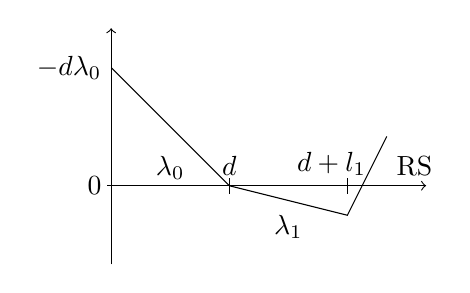
\begin{tikzpicture}
\draw[->] (0,-1) -- (0,2);


\draw[->] (-0.05,0) -- (4,0);

\node[left] at (0,0) {$0$};

\draw (1.5,-.1) -- (1.5,.1);
\node[above] at (1.5,0) {$d$};

\draw (3,-.1) -- (3,.1);
\node[above] at (2.8,0) {$d+l_1$};

\node[left] at (0,1.5) {$-d \lambda_0$};

\draw (0,1.5)-- (1.5,0) -- (3,-.375)-- (3.5,.625);
\node[below] at (.75,0.5) {$\lambda_0$};
\node[below] at (2.25,-0.25) {$\lambda_1$};
\node[right] at (3.5,0.25) {$\RS$};
\end{tikzpicture}
\end{deftn}

\subsubsection{Proof of the Main Theorem}

{\bf Initial Newton polygons}

\begin{lem}
$\NP(R_0)=\NP(S_0)$:
\[ \NP (R_0)=\NP(S_0)=(\lambda_1-\lambda_0)- d \lambda_0+(d-1)\slp( \lambda_0). \]

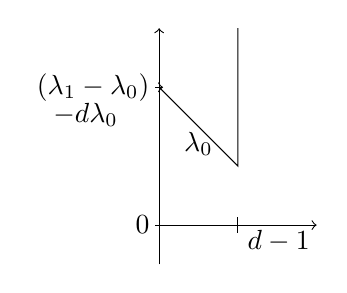
\begin{tikzpicture}
\draw[->] (0,-.5) -- (0,2.5);


\draw[->] (-0.05,0) -- (2,0);

\draw[->] (-0.05,1.75) -- (.05,1.75);
\node[left] at (0,1.75) {$(\lambda_1-\lambda_0)$};
\node[left] at (-.4,1.4) {$-d \lambda_0$};



\node[left] at (0,0) {$0$};


\draw (1,-.1) -- (1,.1);
\node[below, right] at (1,-.2) {$d-1$};


\draw (0,1.75) -- (1,.75) -- (1,2.5);
\node[below] at (.5,1.3) {$\lambda_0$};
\end{tikzpicture}

$\NP (1-V_0B_0 \% A_0)$:
\begin{align*}
\NP ((1-V_0B_0)\% A_0) &\geq (\lambda_1-\lambda_0)+1\slp( \lambda_0)+(d-1) \slp(\lambda_1), \\
&\geq (\lambda_1-\lambda_0)+d\slp( \lambda_0). \\
\end{align*} 
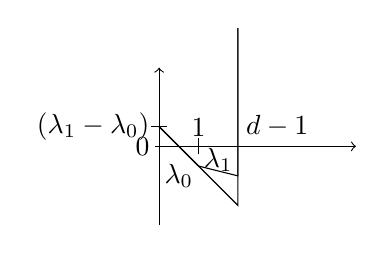
\begin{tikzpicture}
\draw[->] (0,-1) -- (0,1);


\draw[->] (-0.05,0) -- (2.5,0);

\node[left] at (0,0) {$0$};


\node[above] at (1.5,0) {$d-1$};

\draw (.5,-.1) -- (.5,.1);
\node[above] at (.5,0) {$1$};

\draw (-.1,.25) -- (.1,.25);
\node[left] at (0,.25) {$(\lambda_1-\lambda_0)$};

\draw (0,.25) -- (.5,-.25) -- (1,-.375)-- (1,1.5);
\draw (0,.25) -- (.5,-.25) -- (1,-.75)-- (1,1.5);



\node[below] at (.25,-0.1) {$\lambda_0$};
\node[below] at (.75,0.1) {$\lambda_1$};
\end{tikzpicture}


\label{lem:initial_NP}
\end{lem}
\begin{proof}
Clear by Theorem \ref{theo:EDivisionNP}, and the fact that $coeff(P,d)=1.$
\end{proof}

\medskip

{\bf Unchanged Newton polygons}


\begin{lem} \label{lem_unchanged_NP}
$\NP (V_i)$ for $i>0$ ($V_0=1$):
\[\NP(V_i)=0+(d-1)\slp( \lambda_1). \]

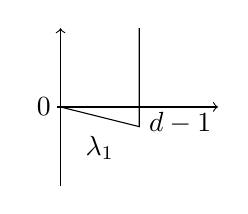
\begin{tikzpicture}
\draw[->] (0,-1) -- (0,1);


\draw[->] (-0.05,0) -- (2,0);

\node[left] at (0,0) {$0$};

\node[below, right] at (1,-.2) {$d-1$};


\draw (0,0) -- (1,-.25) -- (1,1);
\node[below] at (.5,-0.25) {$\lambda_1$};
\end{tikzpicture}

$\NP (B_i)$:
\[\NP(B_i)=0+(l_1)\slp( \lambda_1)+\RS. \]

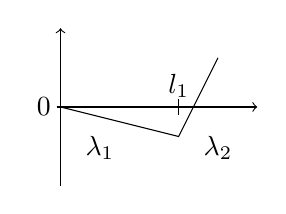
\begin{tikzpicture}
\draw[->] (0,-1) -- (0,1);


\draw[->] (-0.05,0) -- (2.5,0);

\node[left] at (0,0) {$0$};

\draw (1.5,-.1) -- (1.5,.1);
\node[above] at (1.5,0) {$l_1$};


\draw (0,0) -- (1.5,-.375) -- (2,.625);
\node[below] at (.5,-0.25) {$\lambda_1$};
\node[below] at (2,-0.25) {$\lambda_2$};
\end{tikzpicture}

$\NP (A_i)$:
\[\NP(A_i)=-d \lambda_0+d \slp( \lambda_0). \]

\begin{tikzpicture}
\draw[->] (0,-1) -- (0,2);


\draw[->] (-0.05,0) -- (2,0);

\node[left] at (0,0) {$0$};

\draw (1.5,-.1) -- (1.5,.1);
\node[above] at (1.5,0) {$d$};


\node[left] at (0,1.5) {$-d \lambda_0$};

\draw (0,1.5)-- (1.5,0) ;
\node[below] at (.75,0.5) {$\lambda_0$};
\end{tikzpicture}
\end{lem}

\medskip

{\bf Newton polygons inside the loop}

\begin{lem} \label{lem:iteration_inside_the_loop}
\begin{align*}
\NP (R_i), \NP(S_i) & \geq -\lambda_0+2^i(\lambda_1-\lambda_0)+(d-1) \slp (\lambda_0), \\
\NP (1-V_i B_i) & \geq 2^i (\lambda_1-\lambda_0)+(d-1) \slp (\lambda_0),\\
\end{align*}
\end{lem}

We prove the last two lemmas by induction.

\begin{proof}
The case $i=0$ is clear thanks to Theorem \ref{theo:EDivisionNP} and Lemma \ref{lem:initial_NP}.

Now, we assume that for some $i \geq 0$ the formulae defined in the Lemmae \ref{lem_unchanged_NP} and \ref{lem:iteration_inside_the_loop} are satisfied. 
We prove them for $i+1$.

Firstly, thanks to the minoration on $\NP (R_i)$ and the fact that $R_i=A_{i+1}-A_i$, we have $\NP (A_{i+1}= \NP (A_i).$
Since $B_{i+1} = P \div A_{i+1},$ we have $\NP (B_{i+1}) = \NP (B_i).$
We apply \eqref{eqdef:Biminus} to obtain 
\[\NP (B_i-B_{i+1})  \geq 2^i (\lambda_1-\lambda_0)+(\lambda_1-\lambda_0)+(l_1-1) \slp (\lambda_1)+\RS. \]
Then, we can apply \eqref{eqdef:Siminus} to obtain 
\[\NP (S_i-S_{i+1})  \geq -\lambda_0 d+2^i (\lambda_1-\lambda_0)+(d-1) \slp (\lambda_0).\]

As a consequence, we get that $\NP (S_{i+1}) \geq \NP (S_i)$ (pointwise).

Now, we can apply \eqref{eqdef:Viminus} to obtain that 
\[\NP (V_i-V_{i+1}) \geq 2^i (\lambda_1-\lambda_0)+(d-1) \slp (\lambda_0).\]
As a consequence, we get that $\NP(V_i)=\NP(V_{i+1}).$
Similarly, we use \eqref{eqdef:Qiminus} to obtain that
\[\NP (1-Q_i)  \geq  2^i (\lambda_1-\lambda_0)+(d-1) \slp (\lambda_0).\]

This is enough to conclude on the Newton polygon of $R_{i+1}.$
Indeed, thanks to \eqref{eq:Riplus}, we obtain that 
\[\NP (R_i) \geq -\lambda_0+2^i(\lambda_1-\lambda_0)+(d-1) \slp (\lambda_0). \]
We can proceed similarly for $1-V_{i+1} B_{i+1}$ using \eqref{eq:ViBiplus}.

Finally, we can apply \eqref{eqdef:Si2} for $i+1,$
\[S_{i+1} = (B_{i+1} R_{i+1} + (1-V_{i+1} B_{i+1}) S_{i}+(1-V_{i+1} B_{i+1})(S_{i+1}-S_{i})) \% A_{i+1},\] to obtain the desired minoration on $\NP (S_{i+1}).$ This concludes the proof.
\end{proof}

\subsection{A slope factorization algorithm}

Let $P \in K_n[X]$ and $d$ be the abscissa of an extremal point of 
$\NP(P)$. Previously (\emph{cf} Theorem~\ref{theo:slope-factor}), we 
have defined a sequence $(A_i, V_i)$ converging to $(A,V)$ where $A$ is 
a factor of $P$ whose Newton function is $\NF(P)_{|[0,d]}$ and $V$ is the inverse of $B = P/A$ modulo $A$.
We now assume that $P$ is known up to some finite precision: $P = P_0 + 
O(\hspace{0.5mm}\cdots)$ where the object inside the $O$ depends on the 
chosen precision model. We address the two following questions:
(1)~what is the precision on the factor $A$, and
(2)~how one can compute in practive $A$ at this precision?

In the sequel, it will be convenient to use a different normalization on 
$A$ and $B$: if $a_d$ is the coefficient of $P$ of degree $d$, we set
$A^{(1)} = a_d^{-1} A$ and $B^{(1)} = a_d B$
so that $A^{(1)}$ is monic and $P = A^{(1)} B^{(1)}$. We shall also 
always assume that $P$ is monic in the sense that its leading
coefficient is \emph{exactly} $1$; the precision datum on $P$ then 
concerns only the coefficients up to degree $n{-}1$. Similarly, noting
that $A^{(1)}$ and $B^{(1)}$ are monic as well, they only carry a
precision datum up to degree $d{-}1$ and $n{-}d{-}1$ respectively.

\medskip

\noindent
{\bf About the first question.}
We first assume that we are working with lattice precision.
The answer to the first question is then given by the theory of 
\cite{padicprec} and is controlled by the differential of the
application sending $P$ to $A^{(1)}$.

\begin{prop}
\label{prop:precA1}
The application $P \mapsto A^{(1)}$ (where $A^{(1)}$ is defined as before) is 
of class $C^1$ in a neighborhood of $P_0$ and its differential 
at $P_0$ is the linear mapping:
$$dP \mapsto dA^{(1)} = (V^{(1)} \: dP) \mod A^{(1)}$$
where $V^{(1)}$ is the inverse of $B^{(1)}$ modulo $A^{(1)}$.
\end{prop}

\begin{proof}
There certain exists a neighborhood $\mathcal U$ of $P_0$ on which the 
Newton polygon does not vary. On $\mathcal U$, the function $f : P 
\mapsto (A^{(1)},B^{(1)})$ is well defined. It is furthermore bijective 
and its inverse $g$ is given by $(A^{(1)},B^{(1)}) \mapsto A^{(1)}B^{(1)}$.
Clearly $g$ is of class $C^1$ and its differential is given by
\begin{equation}
\label{eq:dPdAdB}
(dA^{(1)}, dB^{(1)}) \mapsto dP = A^{(1)} \: dB^{(1)} + B^{(1)} \: dA^{(1)}.
\end{equation}
Thanks to Bézout Theorem, it is invertible as soon as $A^{(1)}$ and $B^{(1)}$ are
coprime. This happens on $f(\mathcal U) = g^{-1}(\mathcal U)$ because 
$\NP(A^{(1)})$ and $\NP(B^{(1)})$ do not shape a common slope. As a consequence
$f$ is of class $C^1$ on $\mathcal U$. Moreover, its differential is
obtained by inverting Eq.~\eqref{eq:dPdAdB}. Reducing modulo $A^{(1)}$, we
get $dP \equiv B^{(1)} \: dA^{(1)} \pmod {A^{(1)}}$.
The claimed result follows after having noticed that $dA^{(1)}$
has degree at most $d{-}1$.
\end{proof}

\todo{Derive from Proposition~\ref{prop:precA1} a theoretical
result on Newton precision.}

\medskip

\noindent
{\bf About the second question.}
We now study the problem of the effective computation of $A^{(1)}$.


\end{document}
